\documentclass[tikz]{standalone}
\usepackage{amsmath,amssymb}
\usepackage{tikz}
\usetikzlibrary{
	shapes,
	snakes,
	calc,
	decorations,
	decorations.markings,
	decorations.text,
	decorations.pathreplacing}
	
\begin{document}
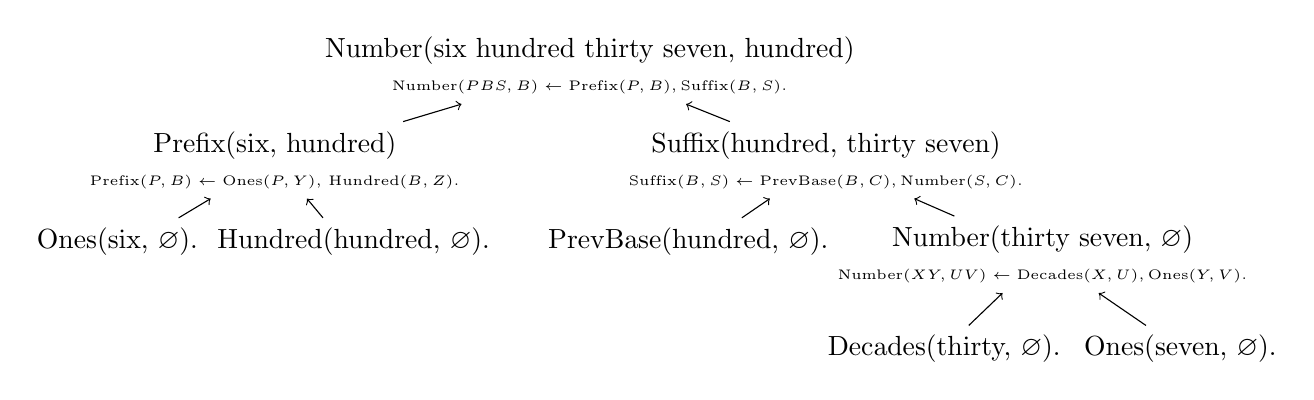
\begin{tikzpicture}[scale=1,auto,every text node part/.style={align=center}]
  
  % Parse Tree
  \node (N0) at (0,2.4) {Number(six hundred thirty seven, hundred)\\
    \tiny$\text{Number}(PBS,B) \leftarrow \text{Prefix}(P,B), \text{Suffix}(B,S).$};
  \node (P1) at (-4,1.2) {Prefix(six, hundred)\\
    \tiny$\text{Prefix}(P,B) \leftarrow \text{Ones}(P,Y),\,\text{Hundred}(B,Z).$};
  \node (S1) at (3,1.2) {Suffix(hundred, thirty seven)\\
    \tiny$\text{Suffix}(B,S) \leftarrow \text{PrevBase}(B,C), \text{Number}(S,C).$};
  \node (O2) at (-6,0) {Ones(six, $\varnothing$).\\};
  \node (H2) at (-3,0) {Hundred(hundred, $\varnothing$).\\};
  \node (PB2) at (1.25,0) {PrevBase(hundred, $\varnothing$).\\};
  \node (N2) at (5.75,0) {Number(thirty seven, $\varnothing$)\\
    \tiny$\text{Number}(XY,UV) \leftarrow \text{Decades}(X,U), \text{Ones}(Y,V).$};
  \node (D3) at (4.5,-1.2) {Decades(thirty, $\varnothing$).};
  \node (O3) at (7.5,-1.2) {Ones(seven, $\varnothing$).};

  \draw [<-] (N0)     to (P1);
  \draw [<-] (N0)  to (S1);
  \draw [<-] (P1)  to (O2);
  \draw [<-] (P1)  to (H2);
  \draw [<-] (S1) to (PB2);
  \draw [<-] (S1) to (N2);
  \draw [<-] (N2) to (D3);
  \draw [<-] (N2) to (O3);
  
\end{tikzpicture}
\end{document}
